\chapter{Estratégia Emocionais}

\section{Estratégia Baseada Modelo OCC}

Tendo em conta as características do modelo emocional \textit{OCC}, foi criada uma estratégia designada com o nome \textit{"Seek and Destroy"}. 
Nesta arquitetura foi tido em conta factores como a quantidade de inimigos, níveis de energias e o número de aliados ainda ativos, para influenciar o estado emocional de cada \textit{robot}. 

Esta tática alicerça-se na existência de um líder, implementado sobre a classe \textit{Seeker} que comanda segundo uma tática os restantes elementos da sua equipa. 
Este outros elementos, identificados pela classe \textit{Destroyer}, caracterizam-se por receber ordens do \textit{Seeker} que representa o comandante da sua equipa. 
\\

Relativamente ao comportamentos dos robots \textit{Seeker}:
\begin{itemize}
    \item O líder da equipa realiza o scan seletivo do terreno (Figura \ref{fig:tact1} (a));
    
    \item Os restantes robots da equipa são descritos pela classe Destroyers.
    
    Este tipo de robots limita-se a apenas a receber ordens do chefe de equipa, tomando uma atitude atacante face aos robots inimigos sobre os quais recebe indicações para flancar/atacar;
    
    \item O líder da equipa, implementado na classe \textit{Seeker}, reconhece a posição e características dos robots da equipa inimiga, através do processo de \textit{scan}. 
    
    Tendo em conta uma determinada características, como o nível de energia, distância ou importância do robots na equipa inimiga, o chefe encaminha os \textit{Destroyers} da sua equipa a atacar este elemento inimigo selecionado. 
    
    \item Caso o líder da equipa esteja sobre fogo inimigo, consoante o seu nível de energia, este pode solicitar proteção aos restantes robots da sua equipa;
    
    \item Idealmente o líder não dispara, apresentando um comportamento passivo e defensivo. 
    
    A sua tarefa principal passa pelo scanning do campo de batalha e deteção dos robots inimigos, podendo com estas informações comandar os restantes elementos da sua equipa. 
    
    Ao não realizar ataques/disparos, o chefe da equipa aumenta ainda as suas probabilidades de se manter ativo durante mais tempo, dado que conserva a sua energia principal;
    
    \item Se todos os Destroyers da equipa morrerem, o líder altera o seu comportamento e estado emocional, assumindo uma posição de ataque face aos restantes inimigos no campo de batalha. 
\end{itemize}

\newpage
\begin{figure}[H]
    \centering
    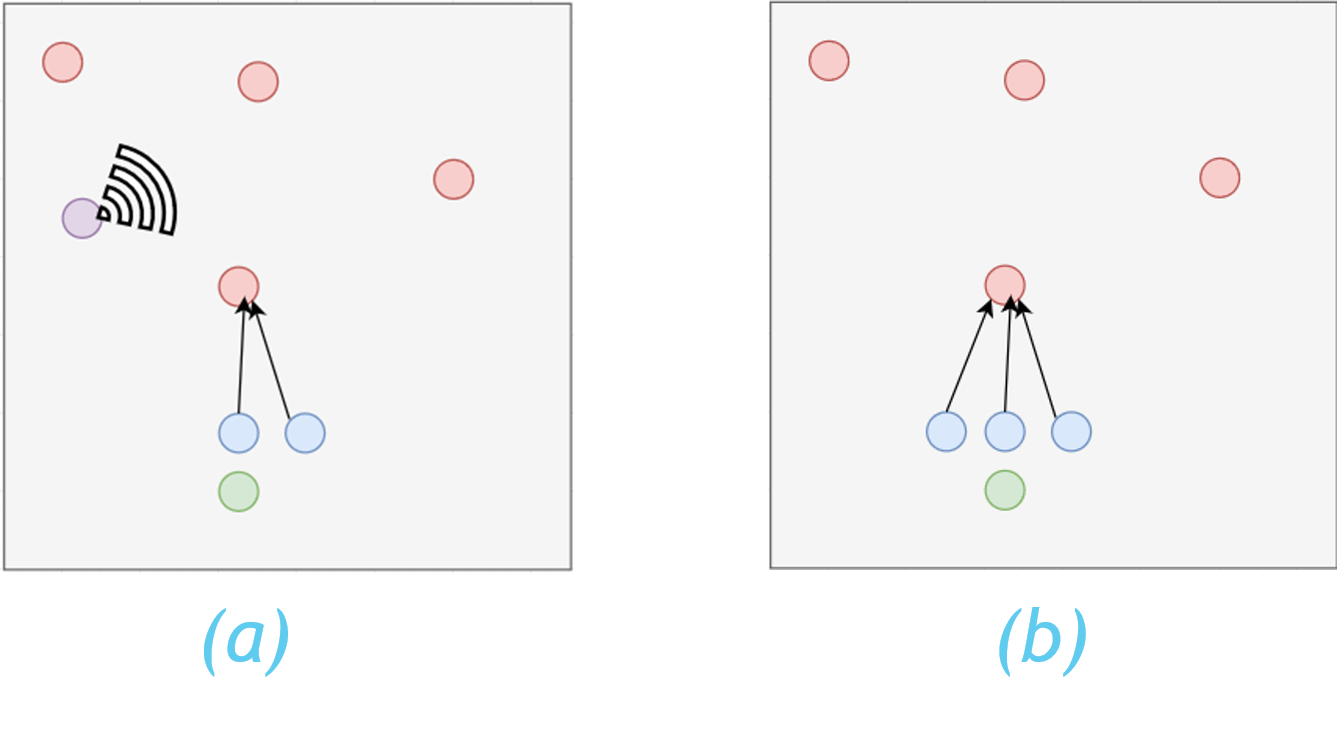
\includegraphics[scale=0.4]{Imagens/Imagem2.png}
    \caption{Esquema (a) Exemplo do Scanning do robot \textit{Seeker} e atribuição de ordens aos robots \textit{Destroyers}; (b) Exemplo do ataque dos robots \textit{Destroyers} após receberem ordens do robot \textit{Seeker}.}
    \label{fig:tact1}
\end{figure}

\begin{figure}[H]
    \centering
    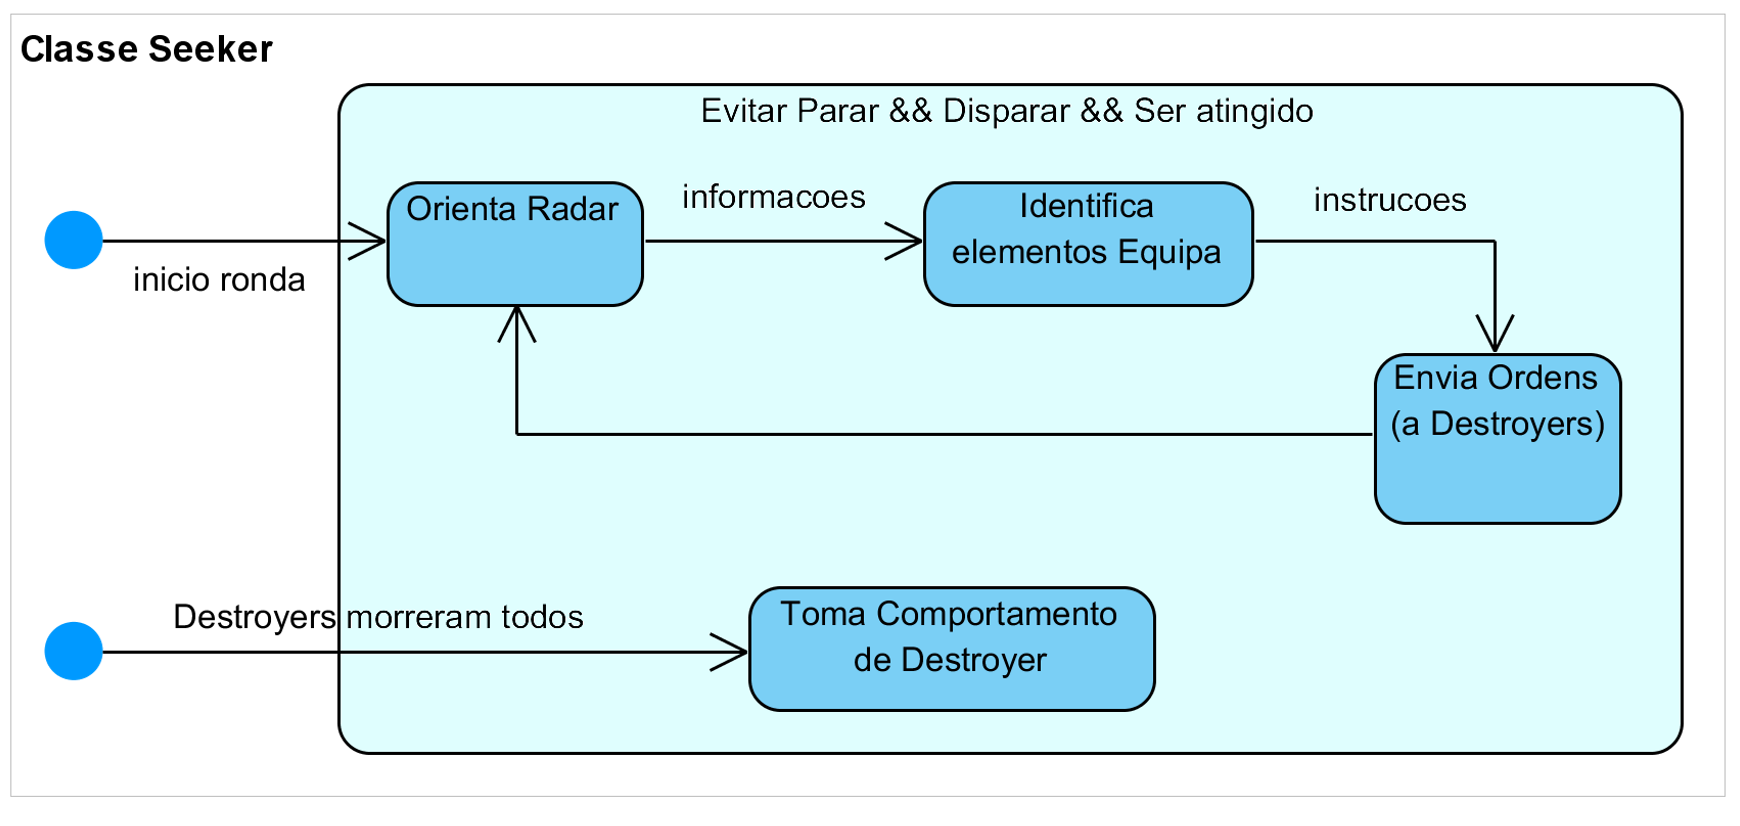
\includegraphics[scale=0.5]{Imagens/evt1.png}
    \label{fig:evet1}
    
    \centering
    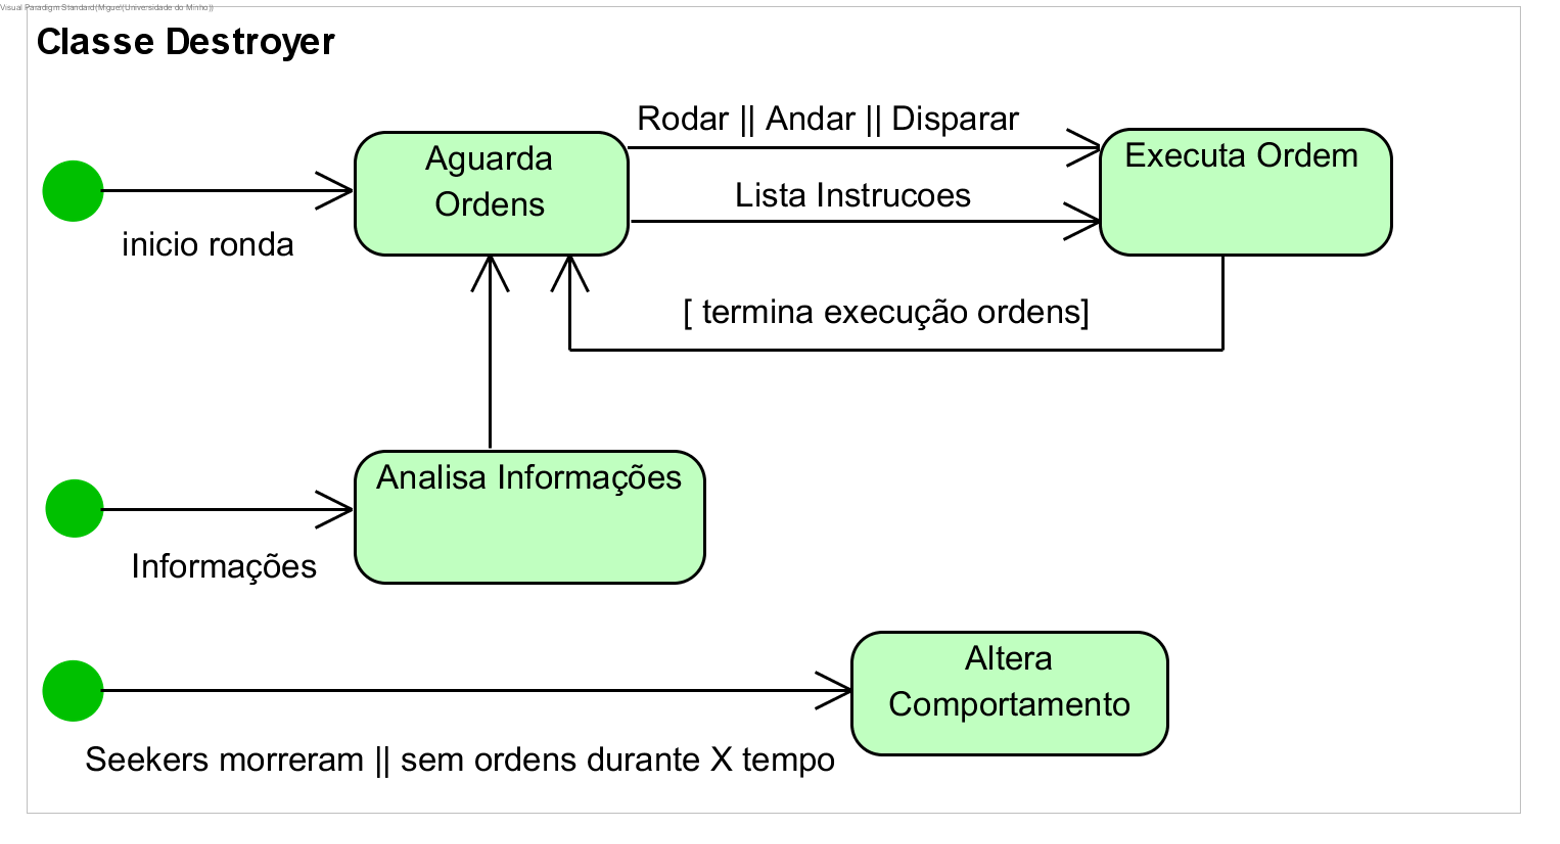
\includegraphics[scale=0.5]{Imagens/evt2.png}
    \caption{Esquema do conjunto de eventos que alteram o estado/comportamento emocional do robot \textit{Seeker} e \textit{Destroyer}.}
    \label{fig:evet2}
\end{figure}
\newpage


Relativamente ao comportamentos dos robots \textit{Destroyer}:
\begin{itemize}
    \item Este tipo de \textit{robots} têm por base a classe \textit{Droid} existente na plataforma \textit{RoboCode}. 
    
    Pela sua simplicidade, estes robots não possuem radares ou qualquer tipo de sensorização do ambiente ou dos robots existentes no ambiente onde se insere.
    Desta forma, as suas ações e tomadas de decisão dependem exclusivamente das informações e instruções recebidas por mensagem por parte do Seeker (chefe) da sua equipa;
    
    \item O seu comportamento é manifestado através das ações que realiza. 
    As ordens recebidas pelo \textit{Seeker} podem ser simples ou pedidos executar uma sequência de instruções;
    
    Ordens simples caracterizam instruções para rodar o robot, deslocar-se, disparar ou atualizar as informações sobre inimigos e pontos do campo de batalha a evitar. 
    Sequências de instruções apresem uma lista com um conjunto das ações anteriormente citadas. 

    \item Se o \textit{Seeker} da equipa for eliminado/destruído, os robots que sigam a classe \textit{Destroyers} deixam de receber ordens que permitam o sucesso global da equipa. 
    
    Assim, como forma de evitar que os mesmos fiquem parados no campo de batalha, os robots apresentam a capacidade de alterar o seu comportamento. Esta mudança ocorre quando deixam de receber ordens do robot líder durante um determinado período de tempo ou, quando verificam que a energia do \textit{Seeker} se encontra bastante baixa. 
    
    A alteração de comportamento passa por assumir um comportamento mais reativo face aos inimigos restantes.
\end{itemize}

